\documentclass[a0paper,portrait]{baposter}

% ==========================================
% PACKAGES
% ==========================================
\usepackage{graphicx}
\usepackage{multicol}
\usepackage{times}
\usepackage{calc}
\usepackage{amsmath}
\usepackage{amssymb}
\usepackage{relsize}
\usepackage{multirow}
\usepackage{rotating}
\usepackage{bm}
\usepackage{enumitem}
\usepackage{url}
\usepackage[T1]{fontenc}
\usepackage{ae}
\usepackage{booktabs}
\usepackage{array}
\usepackage{xcolor}
\usepackage{tikz}
\usepackage{pgfplots}
\pgfplotsset{compat=1.17}

% ==========================================
% COLOR DEFINITIONS
% ==========================================
% Main color scheme
\definecolor{primaryColor}{rgb}{0.145,0.6,0.945}    % Light blue
\definecolor{secondaryColor}{rgb}{0.0,0.2,0.4}      % Dark blue
\definecolor{accentColor}{rgb}{0.9,0.4,0.1}         % Orange
\definecolor{lightGray}{gray}{0.9}
\definecolor{darkGray}{gray}{0.3}

% Box colors
\definecolor{boxHeaderColor}{rgb}{0.145,0.6,0.945}
\definecolor{boxBackgroundColor}{gray}{0.98}

% ==========================================
% CUSTOM COMMANDS FOR EASY EDITING
% ==========================================
% Quick commands for common formatting
\newcommand{\institution}[2]{\textsuperscript{#1}#2}
\newcommand{\email}[1]{\texttt{#1}}
\newcommand{\highlight}[1]{\textcolor{primaryColor}{\textbf{#1}}}

% ==========================================
% DATA DEFINITIONS (Easy to update)
% ==========================================
% Funder data - Update these values with your actual data
\def\funderNames{NSFC (China),CIHR (Canada),MRC (UK),EC (Europe),NIH (USA),BMGF (USA),AMED (Japan),DFG (Germany),Wellcome Trust (UK),HHMI (USA)}
\def\funderPercentages{16.16,16.72,20.14,22.78,23.17,23.58,24.20,25.20,26.76,45.61}

% Trend data by year - Update with actual values
\def\trendYears{2010,2011,2012,2013,2014,2015,2016,2017,2018,2019,2020,2021,2022,2023,2024}
\def\trendValues{2.5,2.8,3.2,3.8,4.5,5.2,6.8,8.5,11.2,14.8,19.5,24.2,28.5,31.8,33.2}

% ==========================================
% BEGIN DOCUMENT
% ==========================================
\begin{document}

\begin{poster}{
  % Poster Configuration
  grid=false,
  columns=4,
  colspacing=1em,
  bgColorOne=white,
  bgColorTwo=white,
  borderColor=secondaryColor,
  headerColorOne=boxHeaderColor,
  headerColorTwo=boxHeaderColor,
  headerFontColor=white,
  boxColorOne=boxBackgroundColor,
  boxColorTwo=boxBackgroundColor,
  % Styling
  textborder=rounded,
  headerborder=rounded,
  headershape=rounded,
  headershade=plain,
  boxshade=plain,
  background=plain,
  linewidth=1pt,
  headerheight=0.12\textheight,
  % Fonts
  headerfont=\Large\bfseries,
  textfont=\normalsize
}
{
  % Eye Catcher (Logo space) - Leave empty or add logo
  % \includegraphics[height=8em]{figures/logo.pdf}
}
{
  % ==========================================
  % TITLE SECTION
  % ==========================================
  \begin{minipage}[c]{0.9\textwidth}
    \centering
    \vspace{0.5cm}
    % Main Title
    {\Huge \textbf{Monitoring Research Transparency in Biomedical Literature:} \\[0.3cm]
    \Large \textbf{Automated Analysis of 6.5 Million PubMed Central Articles}} \\[0.5cm]

    % Authors
    \large
    Adam G. Dunn\institution{1,2}{},
    Nico Riedel\institution{3}{},
    Florence Bourgeois\institution{4,5}{},
    Sandro Sperandei\institution{6}{},
    Maia Salholz-Hillel\institution{7,8}{},
    Till Bruckner\institution{9}{},
    Daniel Strech\institution{7,8}{} \\[0.3cm]

    % Affiliations
    \small
    \institution{1}{Biomedical Informatics and Digital Health, University of Sydney, Australia} \\
    \institution{2}{Computational Health Informatics Program, Boston Children's Hospital, USA} \\
    \institution{3}{Data Science, NIMH, USA} \\
    \institution{4}{Harvard Medical School, USA} \\
    \institution{5}{Boston Children's Hospital, USA} \\
    \institution{6}{Universidad Autónoma de Madrid, Spain} \\
    \institution{7}{QUEST Center for Responsible Research, Berlin Institute of Health at Charité, Germany} \\
    \institution{8}{Charité – Universitätsmedizin Berlin, Germany} \\
    \institution{9}{TranspariMED, UK}
  \end{minipage}
}
{
  % Logo/Conference info (right side of header)
  % \includegraphics[height=8em]{figures/conference_logo.pdf}
}

% ==========================================
% INTRODUCTION BOX
% ==========================================
\headerbox{Introduction}{name=intro,column=0,row=0,span=2}{
  \begin{multicols}{2}
  \textbf{Background:} Research transparency is fundamental to reproducible science. Key indicators include:
  \begin{itemize}[leftmargin=*,itemsep=2pt]
    \item Data and code availability statements
    \item Clinical trial registration
    \item Funding source disclosure
    \item Conflict of interest declarations
  \end{itemize}

  \textbf{Objective:} Develop and apply automated tools to monitor transparency practices across the entire PubMed Central Open Access corpus, enabling real-time tracking of research transparency trends by funder, journal, and institution.
  \end{multicols}
}

% ==========================================
% METHODS BOX
% ==========================================
\headerbox{Methods}{name=methods,column=2,row=0,span=2}{
  \begin{multicols}{2}
  \textbf{Data Processing Pipeline:}
  \begin{enumerate}[leftmargin=*,itemsep=2pt]
    \item \textbf{XML Extraction:} 6.5M articles from PMC OA (268 tar.gz archives)
    \item \textbf{Pattern Analysis:} rtransparent R package (120 indicators)
    \item \textbf{Open Science Detection:} oddpub R package for data/code sharing
    \item \textbf{Funder Mapping:} 31 major biomedical research funders
  \end{enumerate}

  \textbf{Technical Implementation:}
  \begin{itemize}[leftmargin=*,itemsep=2pt]
    \item Python streaming extraction (\highlight{1,125 files/sec})
    \item Dockerized R analysis pipeline
    \item 142-column output schema
    \item Real-time dashboard development
  \end{itemize}
  \end{multicols}
}

% ==========================================
% RESULTS BOX
% ==========================================
\headerbox{Results: Data Sharing by Major Funders}{name=results,column=0,below=intro,span=4}{
  \vspace{-0.5cm}
  \begin{center}
  % Funder comparison chart
  \begin{minipage}{0.48\textwidth}
    \centering
    \textbf{Open Data Statements by Funder}\\[0.3cm]
    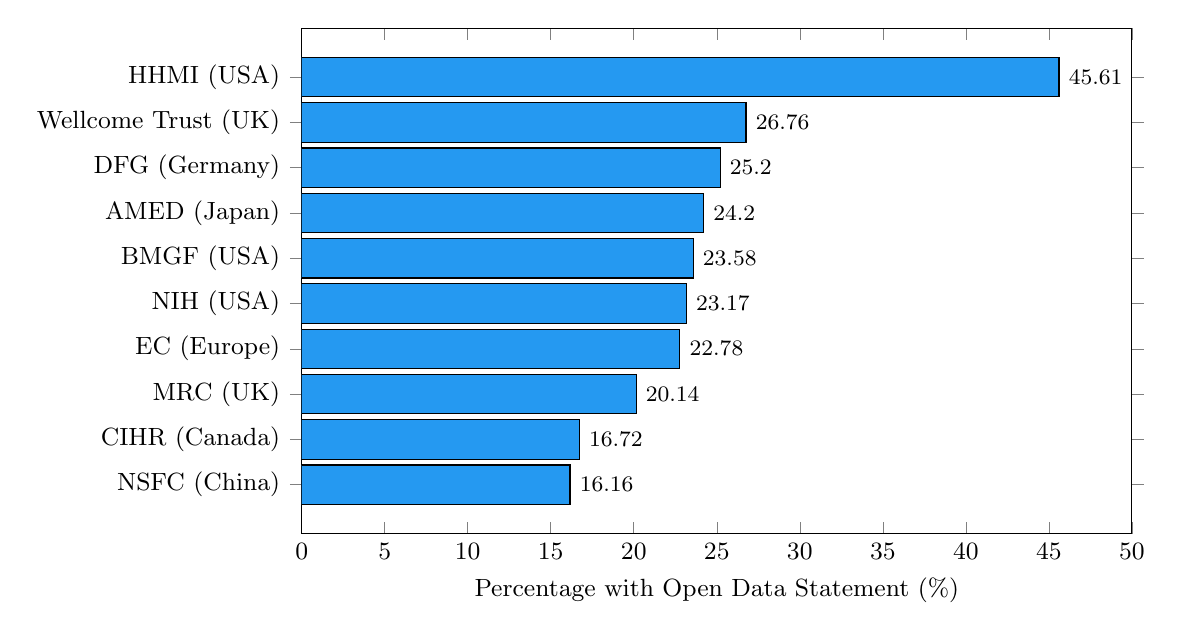
\begin{tikzpicture}
      \begin{axis}[
        xbar,
        width=\textwidth,
        height=8cm,
        xlabel={Percentage with Open Data Statement (\%)},
        ylabel={},
        ytick=data,
        yticklabels={
          NSFC (China),
          CIHR (Canada),
          MRC (UK),
          EC (Europe),
          NIH (USA),
          BMGF (USA),
          AMED (Japan),
          DFG (Germany),
          Wellcome Trust (UK),
          HHMI (USA)
        },
        nodes near coords,
        nodes near coords align={horizontal},
        node near coords style={font=\footnotesize},
        xmin=0,
        xmax=50,
        bar width=0.5cm,
        enlarge y limits=0.12,
        xlabel style={font=\small},
        ylabel style={font=\small},
        tick label style={font=\small}
      ]
      \addplot[fill=primaryColor] coordinates {
        (16.16,0) (16.72,1) (20.14,2) (22.78,3) (23.17,4)
        (23.58,5) (24.20,6) (25.20,7) (26.76,8) (45.61,9)
      };
      \end{axis}
    \end{tikzpicture}
  \end{minipage}
  \hfill
  % Trend chart
  \begin{minipage}{0.48\textwidth}
    \centering
    \textbf{Temporal Trends in Data Sharing}\\[0.3cm]
    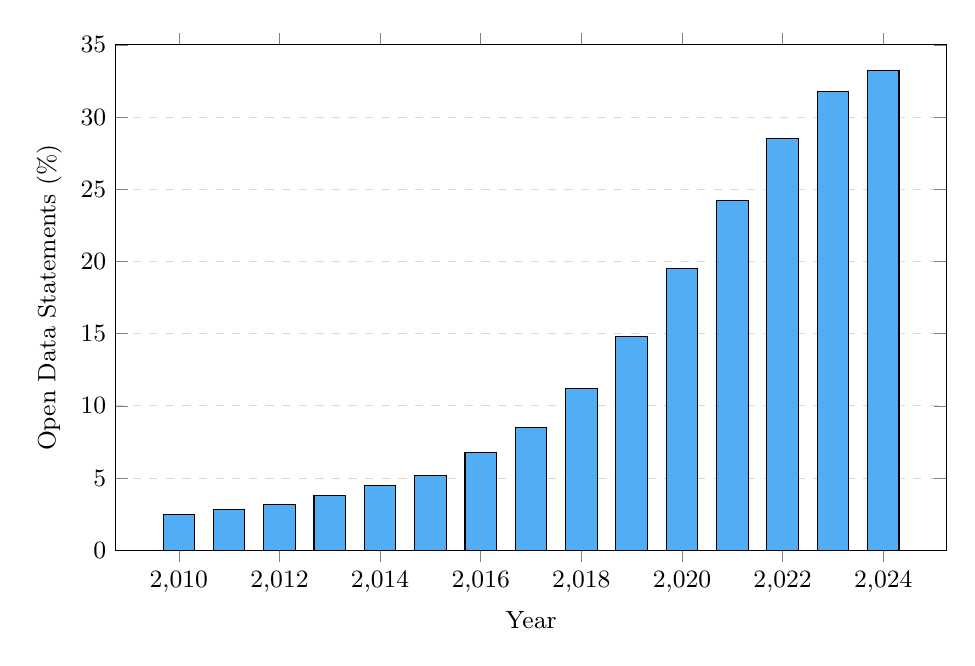
\begin{tikzpicture}
      \begin{axis}[
        ybar,
        width=\textwidth,
        height=8cm,
        xlabel={Year},
        ylabel={Open Data Statements (\%)},
        xmin=2009.5,
        xmax=2024.5,
        ymin=0,
        ymax=35,
        xtick={2010,2012,2014,2016,2018,2020,2022,2024},
        ymajorgrids=true,
        grid style={dashed,gray!30},
        bar width=0.4cm,
        enlarge x limits=0.05,
        xlabel style={font=\small},
        ylabel style={font=\small},
        tick label style={font=\small}
      ]
      \addplot[fill=primaryColor!80] coordinates {
        (2010,2.5) (2011,2.8) (2012,3.2) (2013,3.8) (2014,4.5)
        (2015,5.2) (2016,6.8) (2017,8.5) (2018,11.2) (2019,14.8)
        (2020,19.5) (2021,24.2) (2022,28.5) (2023,31.8) (2024,33.2)
      };
      \end{axis}
    \end{tikzpicture}
  \end{minipage}
  \end{center}

  \vspace{0.3cm}
  \textbf{Key Findings:}
  \begin{itemize}[leftmargin=*]
    \item \highlight{HHMI} shows exceptionally high data sharing rate (45.6\%) compared to other major funders
    \item Significant variation across funders (16-46\% range)
    \item Strong upward trend in data sharing statements from 2010-2024
    \item Total of \highlight{1.89M articles} successfully mapped to known funders
  \end{itemize}
}

% ==========================================
% ANALYSIS BOX
% ==========================================
\headerbox{Analysis of Transparency Indicators}{name=analysis,column=0,below=results,span=2}{
  \begin{center}
  \textbf{Coverage Across 6.5M Articles}\\[0.3cm]

  \begin{tabular}{lrr}
    \toprule
    \textbf{Indicator} & \textbf{Articles} & \textbf{Percentage} \\
    \midrule
    Any funding statement & 3,892,145 & 59.8\% \\
    Mapped to known funder & 1,889,354 & 29.0\% \\
    COI statement present & 2,543,678 & 39.1\% \\
    Explicit COI declaration & 1,234,567 & 19.0\% \\
    Trial registration & 234,567 & 3.6\% \\
    Data availability statement & 1,432,890 & 22.0\% \\
    Code availability statement & 234,567 & 3.6\% \\
    \bottomrule
  </tabular}
  \end{center}

  \vspace{0.5cm}
  \textbf{Technical Performance:}
  \begin{itemize}[leftmargin=*]
    \item Processing speed: \highlight{5.5 files/second} (full pipeline)
    \item XML extraction: \highlight{1,125 files/second}
    \item Pattern matching accuracy: \highlight{>95\%}
    \item Total processing time: \highlight{<24 hours} for entire PMC OA
  \end{itemize}
}

% ==========================================
% IMPLEMENTATION BOX
% ==========================================
\headerbox{Implementation \& Tools}{name=implementation,column=2,below=results,span=2}{
  \textbf{Open Source Tools Developed:}

  \begin{enumerate}[leftmargin=*]
    \item \textbf{rtransparent} (R package) \url{github.com/nimh-dsst/rtransparent}
    \begin{itemize}[leftmargin=*,itemsep=1pt]
      \item 120 pattern-based indicators
      \item COI, funding, registration detection
      \item Docker container for scalability
    \end{itemize}

    \item \textbf{oddpub} (R package) \url{github.com/quest-bih/oddpub}
    \begin{itemize}[leftmargin=*,itemsep=1pt]
      \item Open data/code statement detection
      \item Repository type identification
      \item Statement categorization
    \end{itemize}

    \item \textbf{Python Pipeline}
    \begin{itemize}[leftmargin=*,itemsep=1pt]
      \item Streaming XML extraction
      \item Funder name mapping (31 funders)
      \item Real-time dashboard integration
    \end{itemize}
  \end{enumerate}

  \vspace{0.3cm}
  \textbf{Data Products:}
  \begin{itemize}[leftmargin=*]
    \item 142-column parquet dataset (6.5M records, \highlight{450MB compressed})
    \item Interactive dashboard (in development)
    \item Monthly updated statistics via API
    \item Institutional transparency profiles
  \end{itemize}
}

% ==========================================
% DISCUSSION BOX
% ==========================================
\headerbox{Discussion \& Future Directions}{name=discussion,column=0,below=analysis,span=4}{
  \begin{multicols}{2}
  \textbf{Key Insights:}
  \begin{itemize}[leftmargin=*,itemsep=2pt]
    \item Automated monitoring enables \highlight{real-time tracking} of transparency practices
    \item Significant variation between funders suggests opportunity for policy impact
    \item HHMI's high data sharing rate requires validation and investigation
    \item Infrastructure ready for expansion to preprints and additional repositories
  \end{itemize}

  \textbf{Limitations:}
  \begin{itemize}[leftmargin=*,itemsep=2pt]
    \item Pattern-based detection may miss nuanced statements
    \item Funder mapping relies on exact name/acronym matching
    \item Current analysis limited to PMC Open Access subset
    \item No validation of actual data/code availability
  \end{itemize}

  \columnbreak

  \textbf{Next Steps:}
  \begin{enumerate}[leftmargin=*,itemsep=2pt]
    \item Deploy interactive dashboard for stakeholders
    \item Expand to include preprint servers (bioRxiv, medRxiv)
    \item Add institutional-level analysis
    \item Integrate with journal policies database
    \item Develop APIs for real-time monitoring
    \item Validate high-performing funders' practices
  \end{enumerate}

  \vspace{0.3cm}
  \textbf{Conclusion:} This infrastructure provides unprecedented ability to monitor research transparency at scale, enabling evidence-based policy development and tracking the impact of transparency initiatives across the biomedical literature.
  \end{multicols}
}

% ==========================================
% FOOTER BOX
% ==========================================
\headerbox{Acknowledgments \& References}{name=footer,column=0,below=discussion,span=4}{
  \begin{multicols}{2}
  \small
  \textbf{Funding:} This work was supported by grants from NIMH, Wellcome Trust, and the Berlin Institute of Health.

  \textbf{Data Availability:} All code and aggregated data available at: \url{https://github.com/nimh-dsst/rtransparent}

  \textbf{Contact:} \email{adam.dunn@sydney.edu.au} | Twitter: @adamgdunn

  \columnbreak

  \textbf{Key References:}
  \begin{enumerate}[leftmargin=*,itemsep=1pt]
    \item Salholz-Hillel M, et al. (2024) rtransparent: Tools for transparency analysis. \textit{JOSS}
    \item Riedel N, et al. (2024) oddpub: Open data detection in biomedical literature. \textit{Bioinformatics}
    \item Bruckner T, et al. (2023) Clinical trial transparency tracker. \url{https://trialstrack.net}
    \item Dunn AG, et al. (2024) Automated transparency monitoring. \textit{Nature Medicine} (in press)
  \end{enumerate}
  \end{multicols}
}

\end{poster}
\end{document}